\begin{flushright} {\tiny {\color{gray} python\_codes/fieldstone\_118/text.tex}} \end{flushright}

\lstinputlisting[language=bash,basicstyle=\small]{python_codes/fieldstone_118/keywords}

\begin{center}
\fbox{\textbf{\huge \color{teal} P}}
Files at \url{https://github.com/cedrict/fieldstone/tree/master/python_codes/fieldstone_118}
\end{center}

\par\noindent\rule{\textwidth}{0.4pt}

%%%%%%%%%%%%%%%%%%%%%%%%%%%%%%%%%%%%%%%%%%%%%%%%%%%%%%%%%%%%%%%%%%%%%%%%%%%%%%%%%%%%%%%%%%%%%%

The setup is taken from \textcite{mato83} (1983) and \textcite{futo85} (1985).
The true motivation here is to replicate the 1985 study 
and have a reason to focus on the following most improbable figure in a peer reviewed
article in geosciences:

\begin{center}
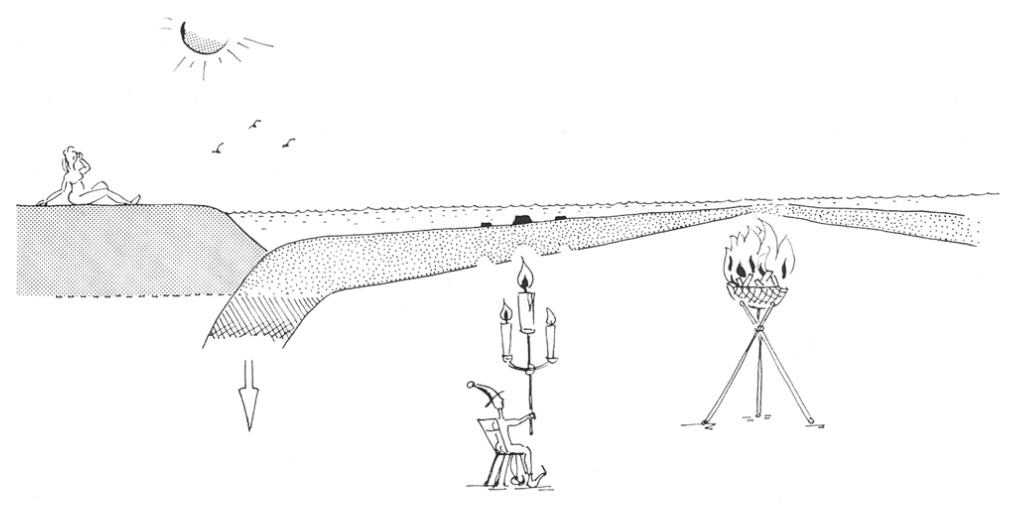
\includegraphics[width=12cm]{./images/interesting/futo85}\\
{\captionfont Taken from \textcite{futo85} (1985).}
\end{center}

In the original paper (1983) the authors solve the incompressible isothermal Stokes equations
with a stream function approach. The resulting equation is solved by means of the
Finite Difference method and the Marker and Cell (MAC) method \cite{hawe65}.

The domain is a 2D Cartesian box of size $L_x \times L_y=(400,180)~\si{\km}$. 
There are three fluids in the domain: 
water ($\rho_w=1030~\si{\kg\per\cubic\meter}$, $\eta_w=10^{-3}~\si{\pascal\second}$), 
lithosphere ($\rho_l=3300~\si{\kg\per\cubic\meter}$, $\eta_l$) and 
asthenosphere ($\rho_a=3200~\si{\kg\per\cubic\meter}$, $\eta_a$).
Boundary conditions are free-slip on all sides of the domain.
Unfortunately the authors do not specify the mesh resolution that was used. 

Six cases are considered\footnote{Note that in the paper all viscosities 
are expressed in Poise, with 1~Poise=0.1~\si{\pascal\second}}:
\begin{center}
\begin{tabular}{lccc}
Case & $\eta_l$ (\si{\pascal\second}) & $\eta_a$  (\si{\pascal\second}) & domain size (\si{\km})\\
\hline
1 & $10^{22}$ & $10^{21}$ & $400\times 180$\\
2 & $10^{22}$ & $10^{20}$ & $400\times 180$\\
3 & $10^{22}$ & $10^{19}$ & $400\times 180$\\
4 & $10^{23}$ & $10^{21}$ & $400\times 180$\\
\hline
5 & $10^{22}$ & $10^{20}$ & $800\times 140$\\
6 & $10^{22}$ & $10^{19}$ & $800\times 140$\\
\hline
\end{tabular}
\end{center}

\begin{center}
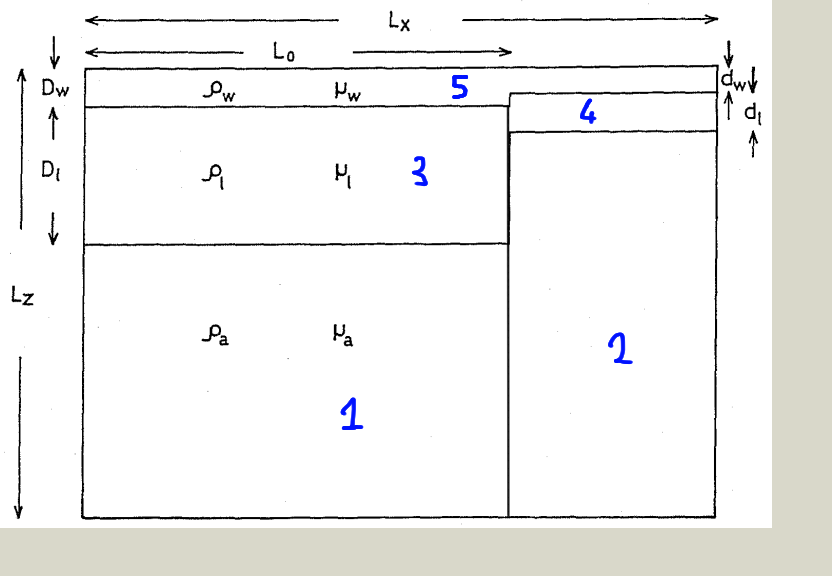
\includegraphics[width=7cm]{python_codes/fieldstone_118/images/mato83}\\
{\captionfont Taken from \textcite{mato83}. Dw=10km, Dl=50km, dw=8km, 
dl=10km, $L_0=3L_x/4$. Blue numbers indicate the numbering of each compositional field.}
\end{center}

Interestingly the authors state: ``The materials are initially placed so that 
uniform hydrostatic pressure holds at the bottom of the calculation area''. 
On the left side, the pressure at the bottom is given by 
\[
p_b=(10\cdot 1030+50\cdot 3300+80\cdot3200)g_y = 431,300g_y
\]
while on the right side it is
\[
p_b=(8\cdot 1030+10\cdot 3300+122 \cdot3200)g_y = 431,640g_y
\]
which means that indeed the system is in isostatic equilibrium at the beginning of the 
simulation. 

The authors use a CFL condition to determine the time step $\delta t$ and use an arithmetic 
averaging scheme for both density and viscosity.

%%%%%%%%%%%%%%%%%%%%%%%%%%%%%%%%%%%%%%%%%%%%%%%%%%%%%%%%%%%%%%%%%%%%%%%
\subsection*{Using Aspect}

I am using here \aspect and the input files are included in the folder (in 
what follows I have used the one based on compositional fields but there
is also a second prm file based on particles). It is straightforward 
since the flow is isothermal and incompressible and the domain a Cartesian box with 
free slip boundary conditions. A pressure normalisation is then necessary to remove 
the pressure nullspace and the pressure is then set to zero on average on the top boundary. 
A CFL condition is used with $C=0.25$ and the models 
are run 50~\si{\mega\year}. 
Two repetitions are used in the horizontal directions so that elements are almost square.
The mesh counts $128\times 64=8192$ cells, i.e. a resolution of about 3~\si{\km} which is barely enough to 
accurately follow the thin lithosphere.


%%%%%%%%%%%%%%%%%%%%%%%%%%%%%%%%%%%%%%%%%%%%%%%%%%%%%%%%%%%%%%%%%%%%%%%
\subsection*{This stone (instantaneous)}

I have also written a $Q_2\times Q_1$ code which is able to 
compute the solution of the problem at $t=0$ (it stems from \stone 40). 
It does not feature any algorithm to advect interfaces or fluids and
it is also quite naive and relies on full matrices for the 
blocks of the Stokes matrix. Nevertheless, it allows to compute the solution 
on a $80\times 90$ mesh, i.e. a $5\times 2~\si{\km}$ resolution with 
all fluid boundaries alligned with mesh boundaries:

\begin{center}
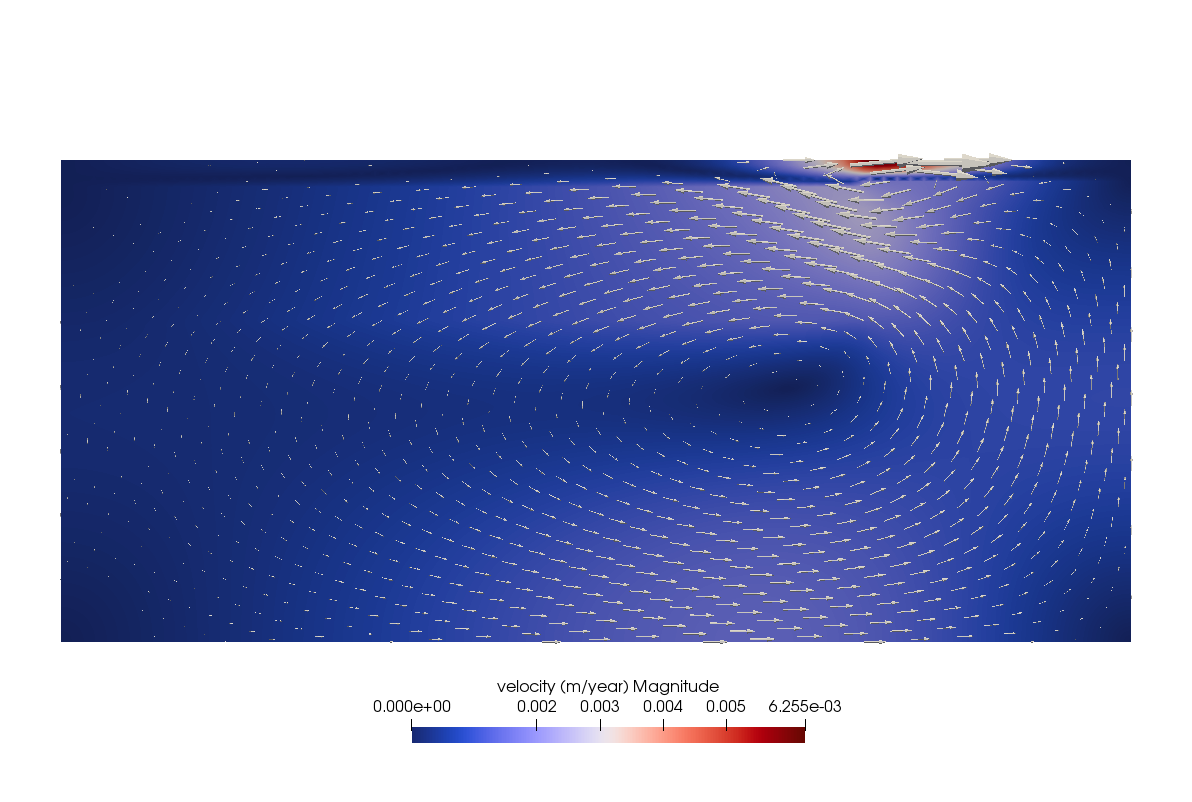
\includegraphics[width=5.6cm]{python_codes/fieldstone_118/results/case1/stone/vel}
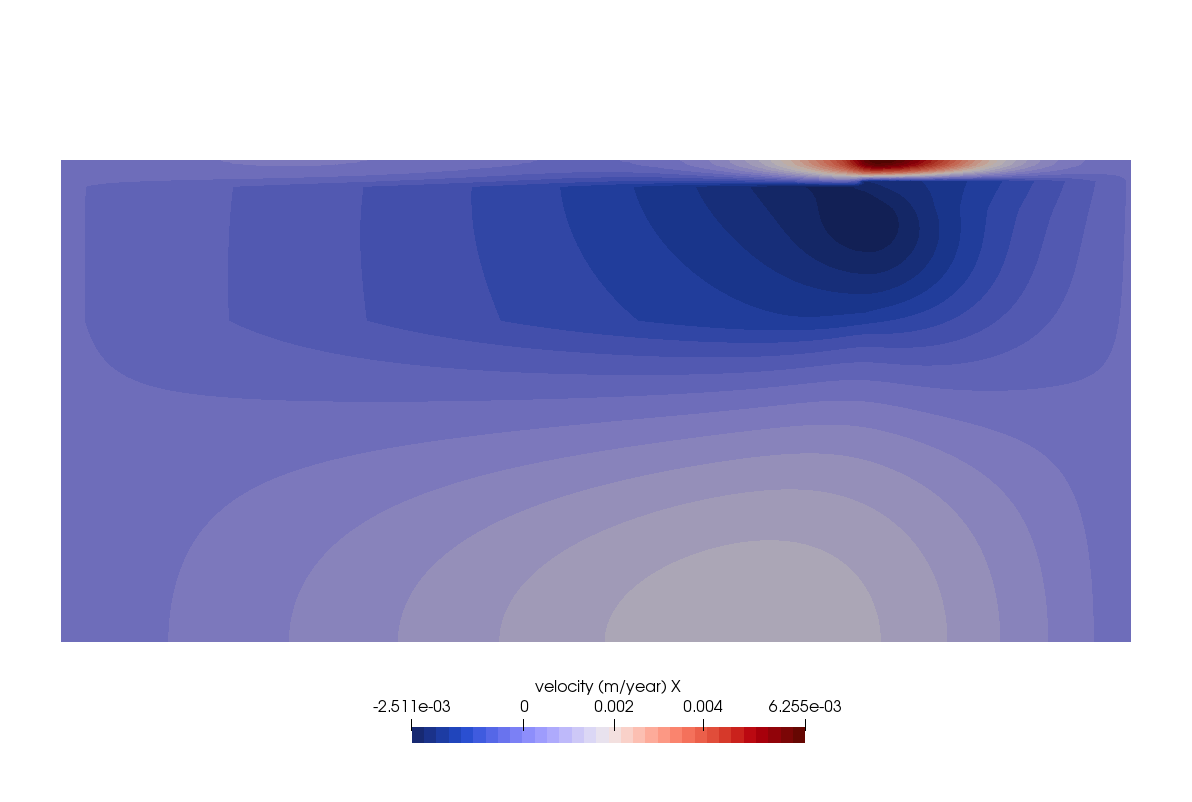
\includegraphics[width=5.6cm]{python_codes/fieldstone_118/results/case1/stone/u}
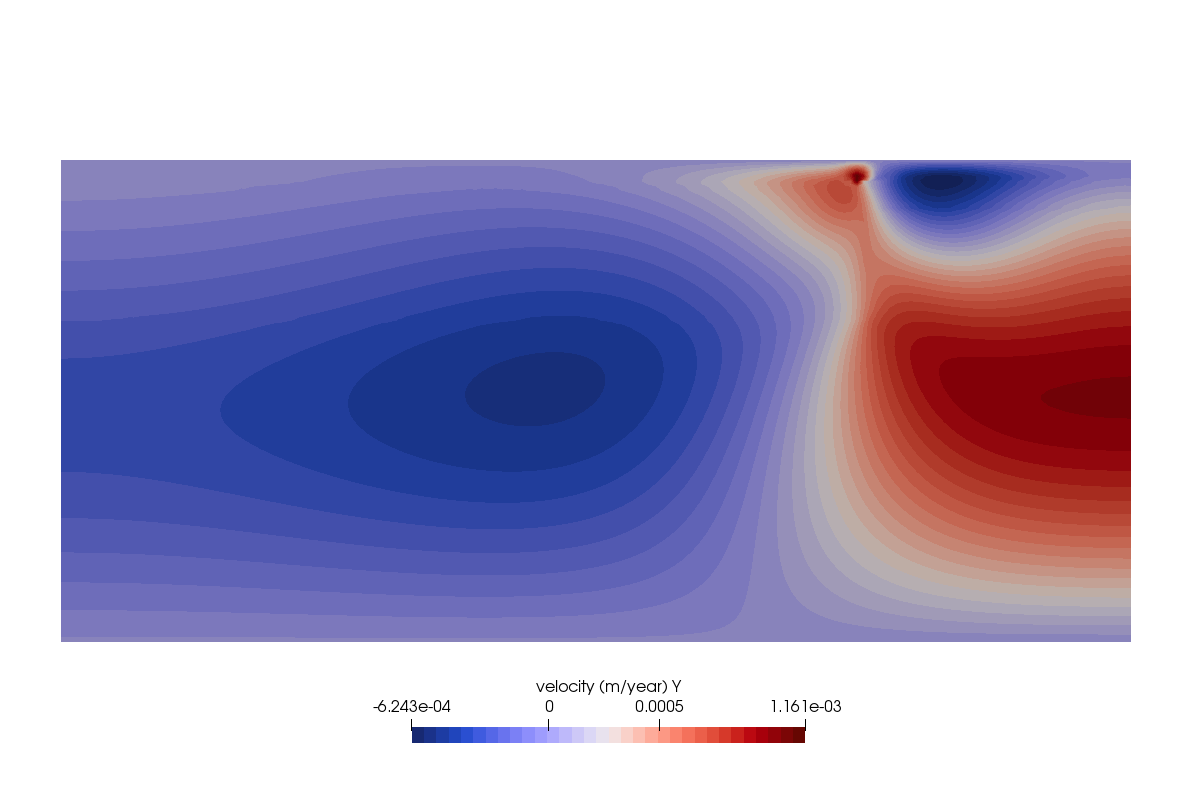
\includegraphics[width=5.6cm]{python_codes/fieldstone_118/results/case1/stone/v}\\
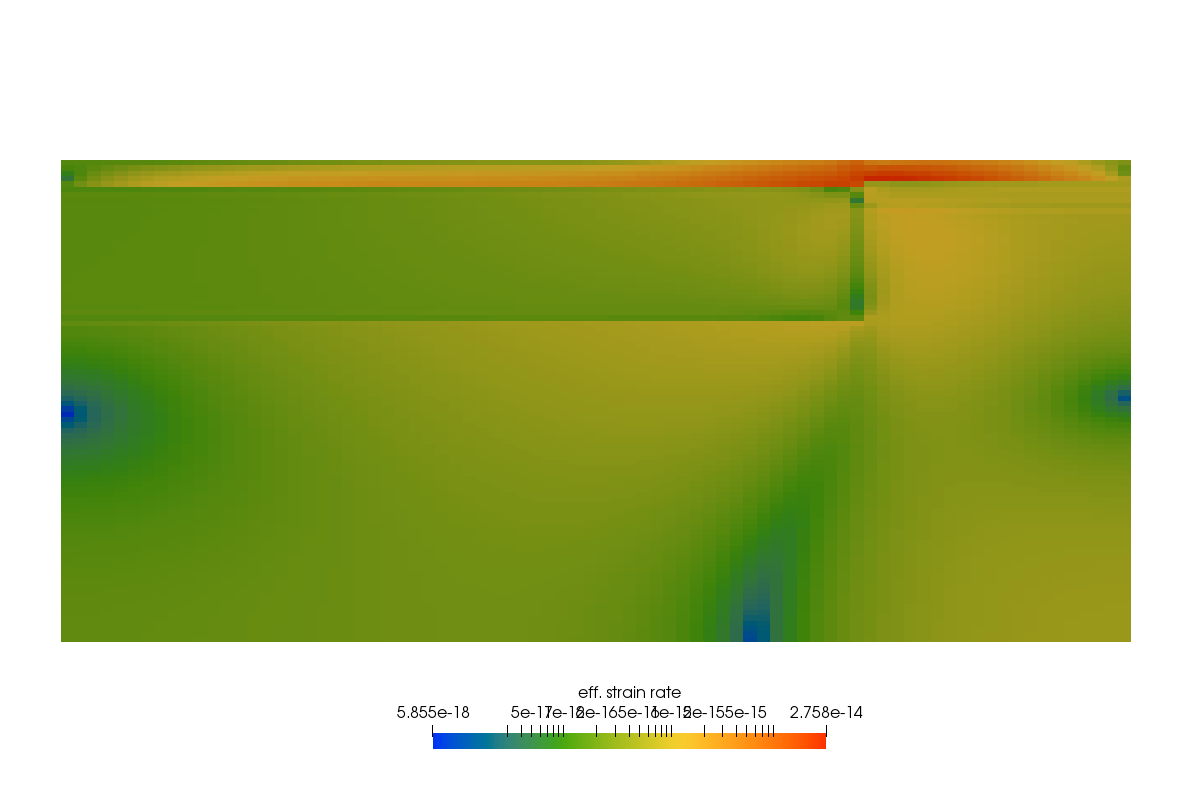
\includegraphics[width=5.6cm]{python_codes/fieldstone_118/results/case1/stone/sr}
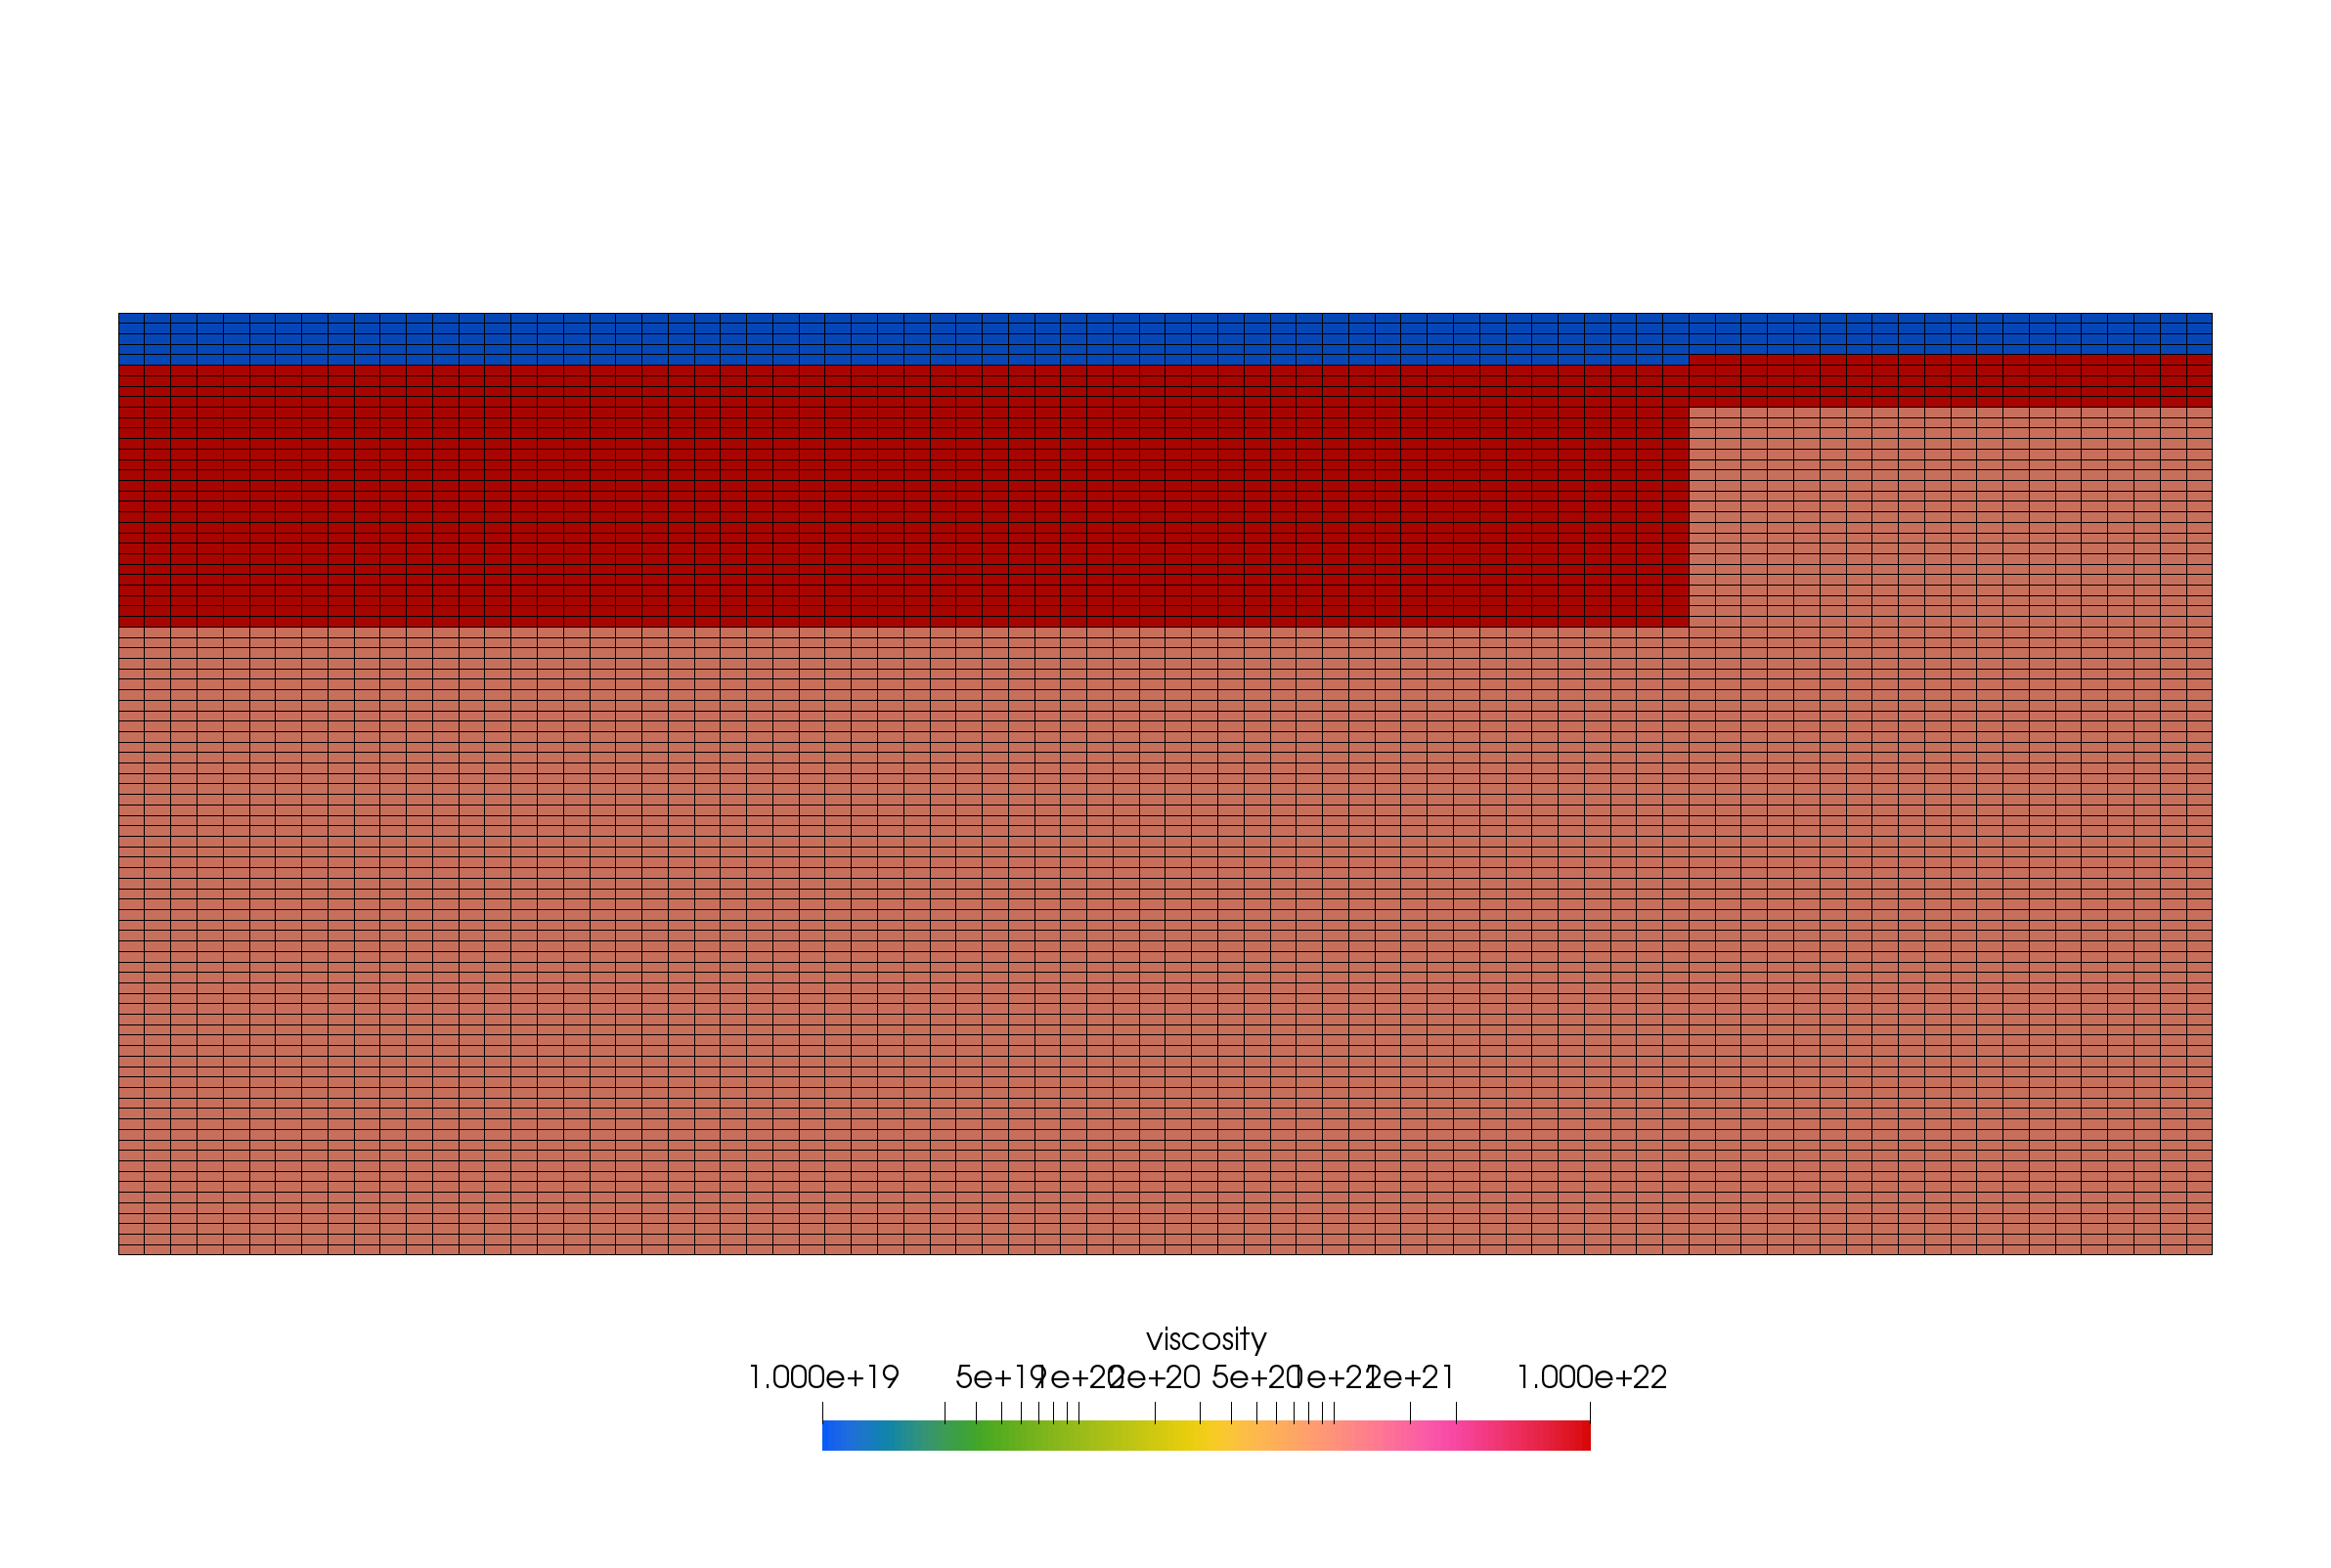
\includegraphics[width=5.6cm]{python_codes/fieldstone_118/results/case1/stone/eta}
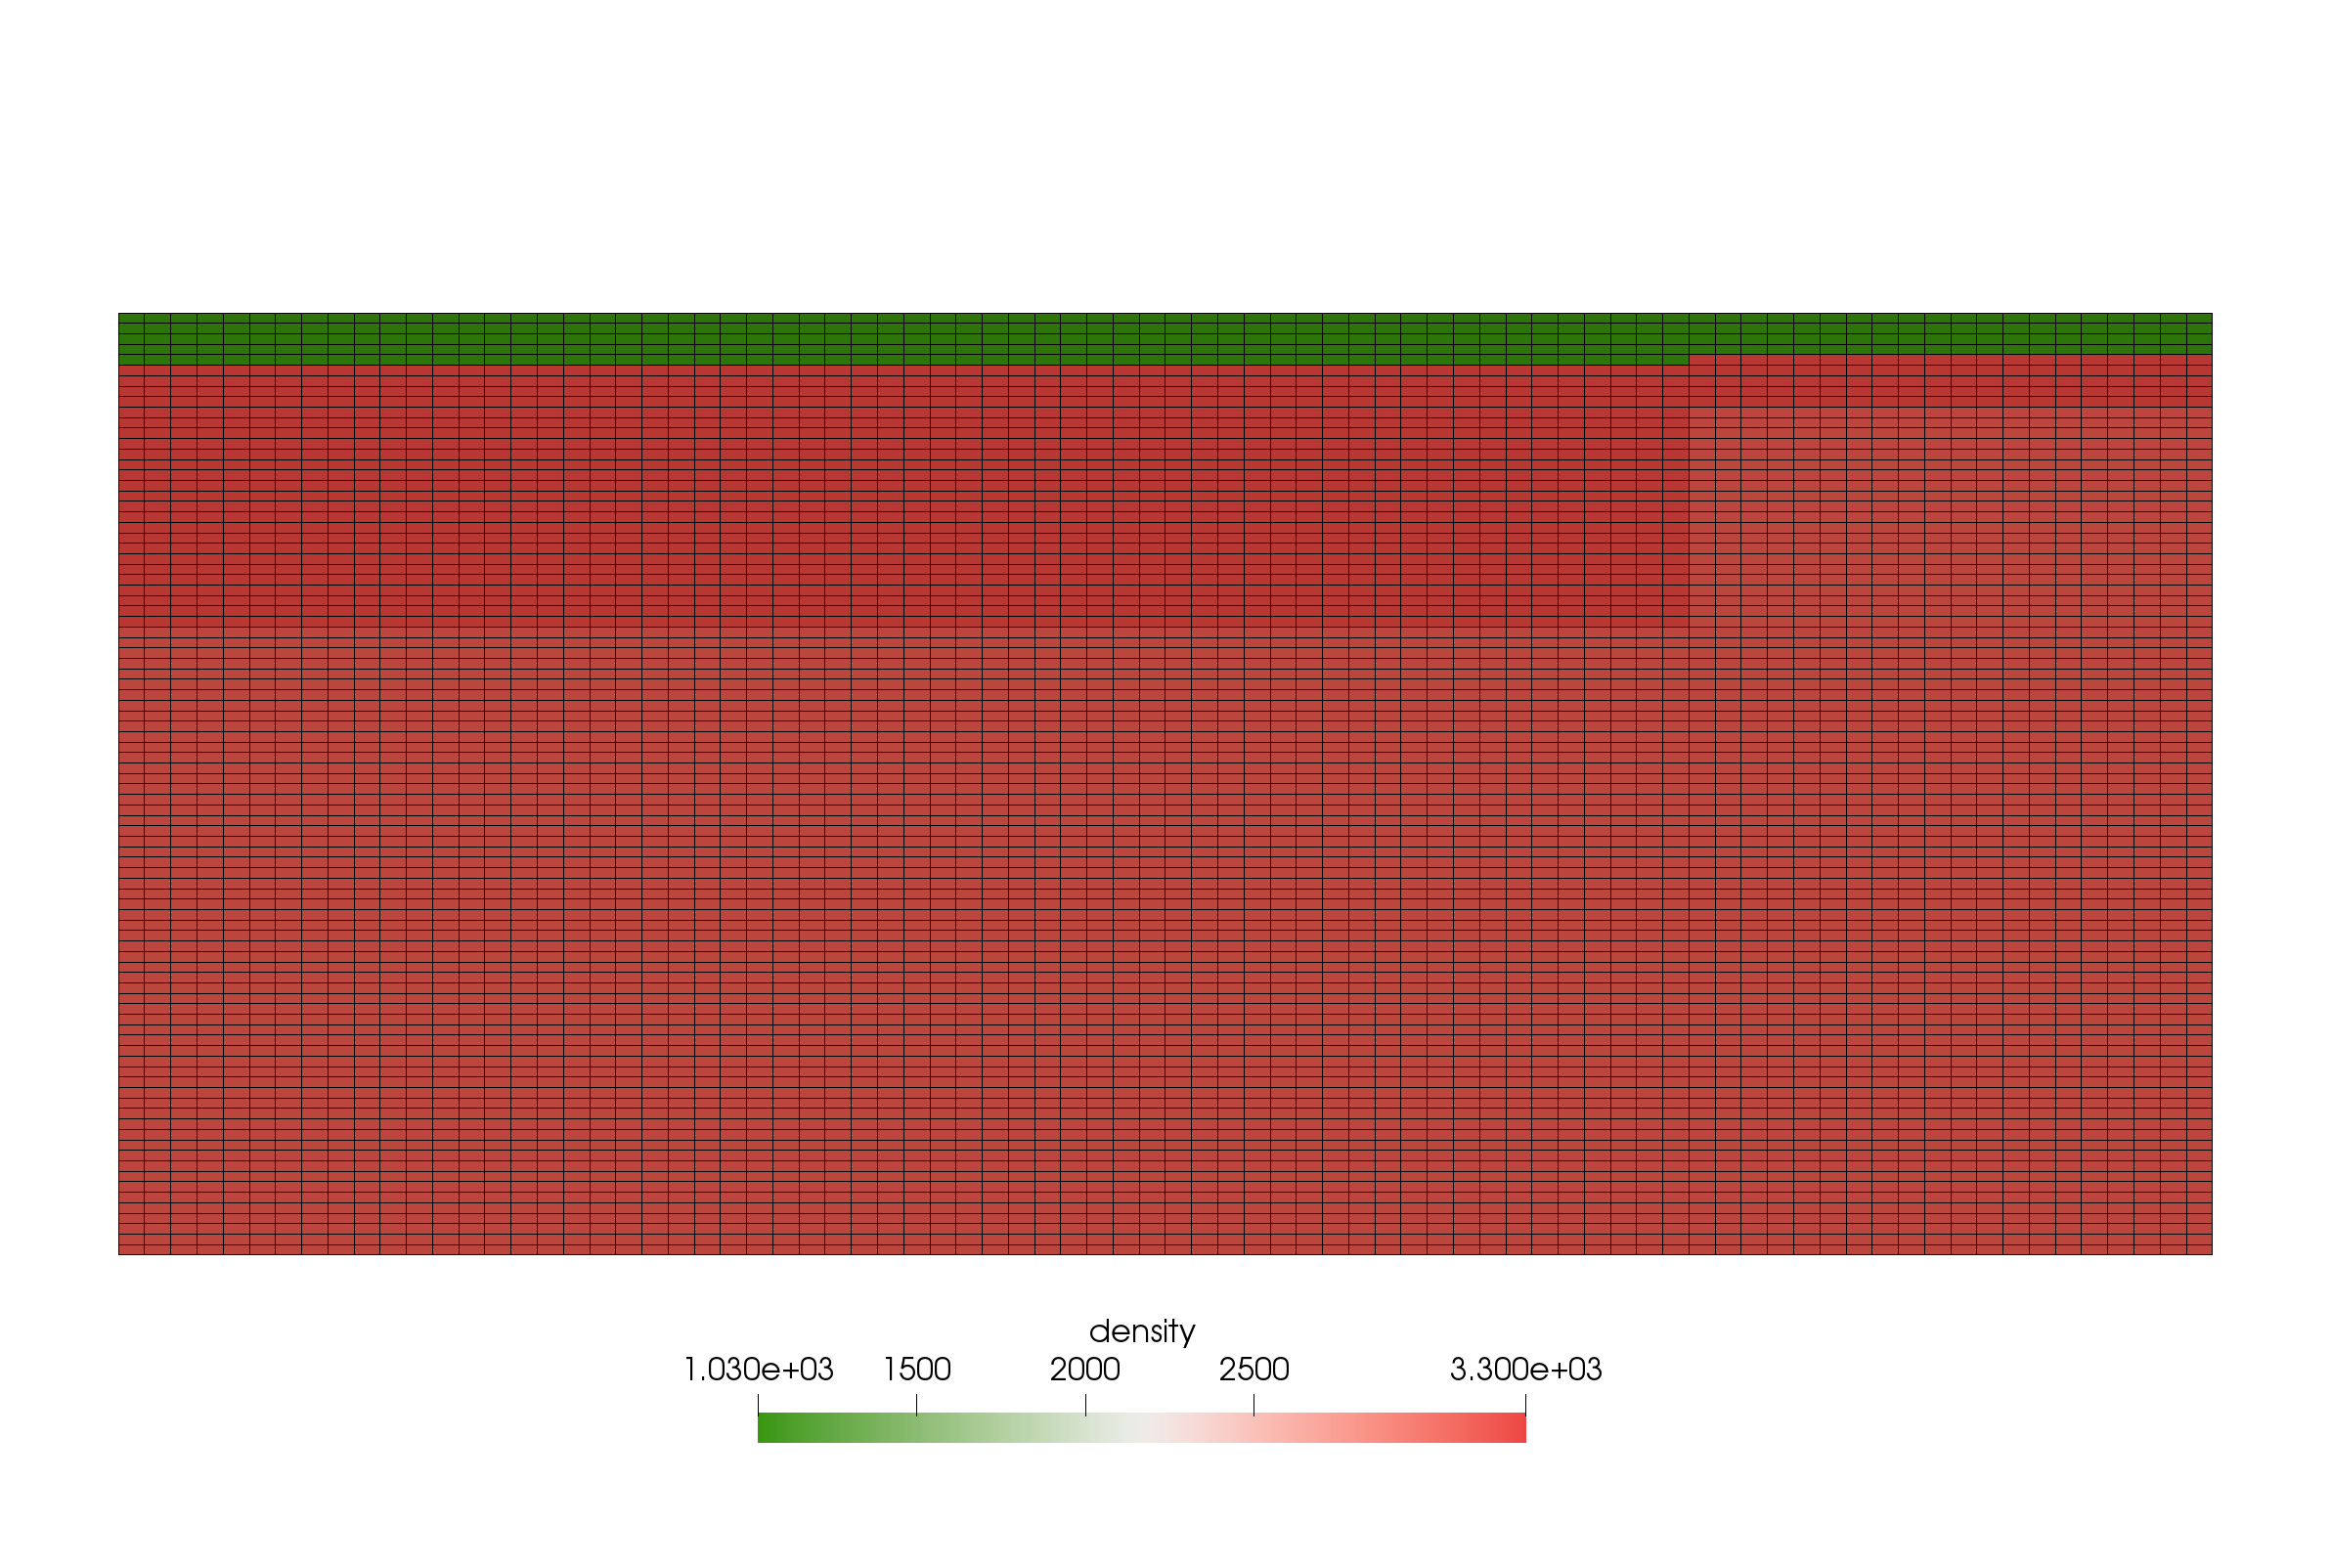
\includegraphics[width=5.6cm]{python_codes/fieldstone_118/results/case1/stone/rho}\\
{\captionfont Results obtained with this \stone, resolution  $80\times 90$ for Case 1.}
\end{center}

\newpage

%%%%%%%%%%%%%%%%%%%%%%%%%%%%%%%%%%%%%%%%%%%%%%%%%%%%%%%%%%%%%%%%%%%%%%%
\subsection*{Results - Case 1}

Results obtained with \aspect agree nicely with those of the paper
although the water layer and the thin lithosphere is much more 
deformed in their case. The run took approx. 6500~s to complete on a single core.

\begin{center}
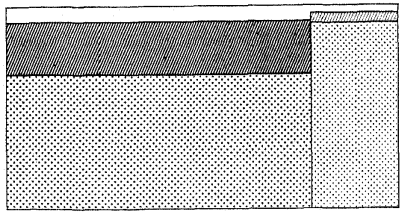
\includegraphics[width=3.25cm]{python_codes/fieldstone_118/images/case1/a}
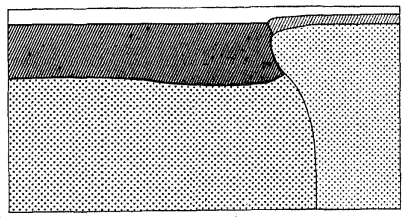
\includegraphics[width=3.25cm]{python_codes/fieldstone_118/images/case1/b}
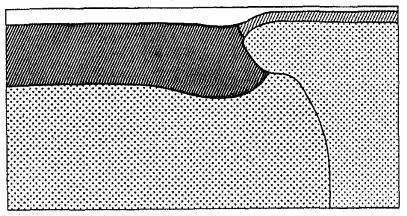
\includegraphics[width=3.25cm]{python_codes/fieldstone_118/images/case1/c}
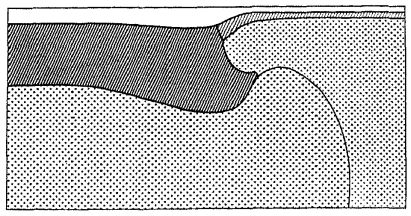
\includegraphics[width=3.25cm]{python_codes/fieldstone_118/images/case1/d}
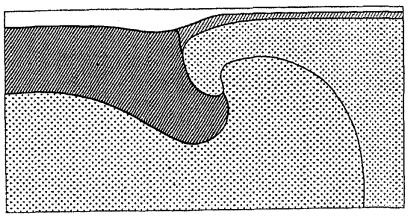
\includegraphics[width=3.25cm]{python_codes/fieldstone_118/images/case1/e}\\

\includegraphics[width=3.25cm]{python_codes/fieldstone_118/results/case1/a}
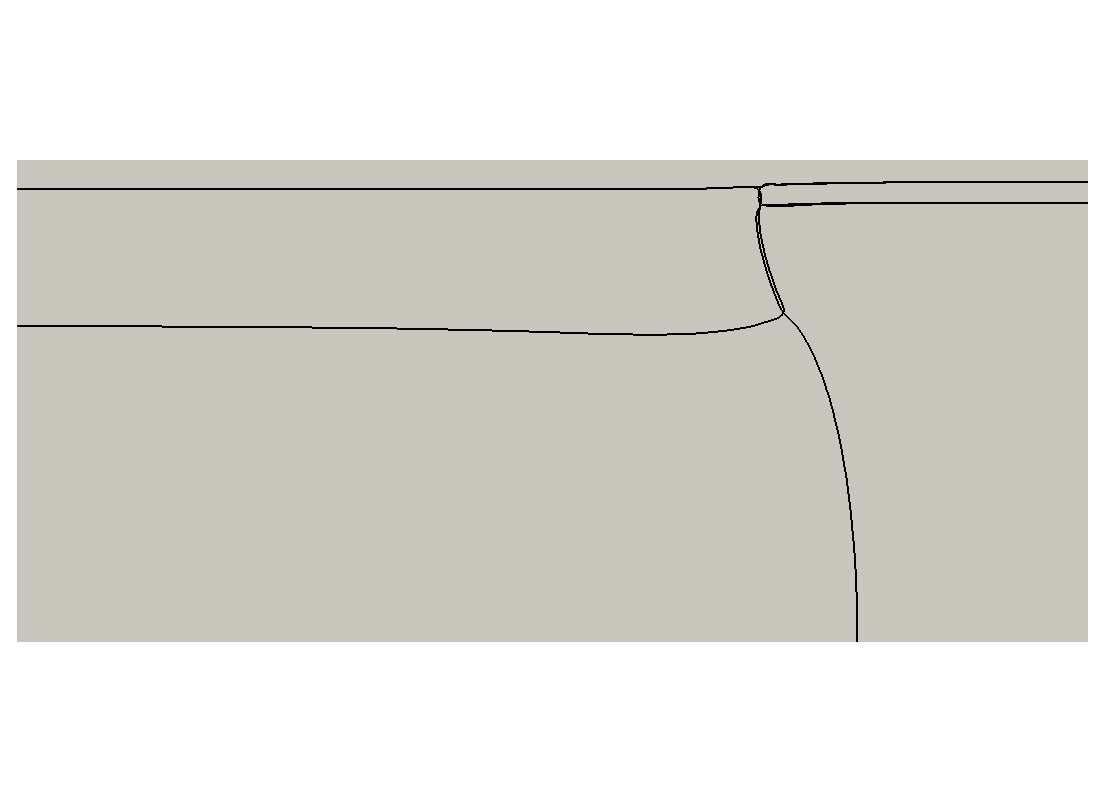
\includegraphics[width=3.25cm]{python_codes/fieldstone_118/results/case1/b}
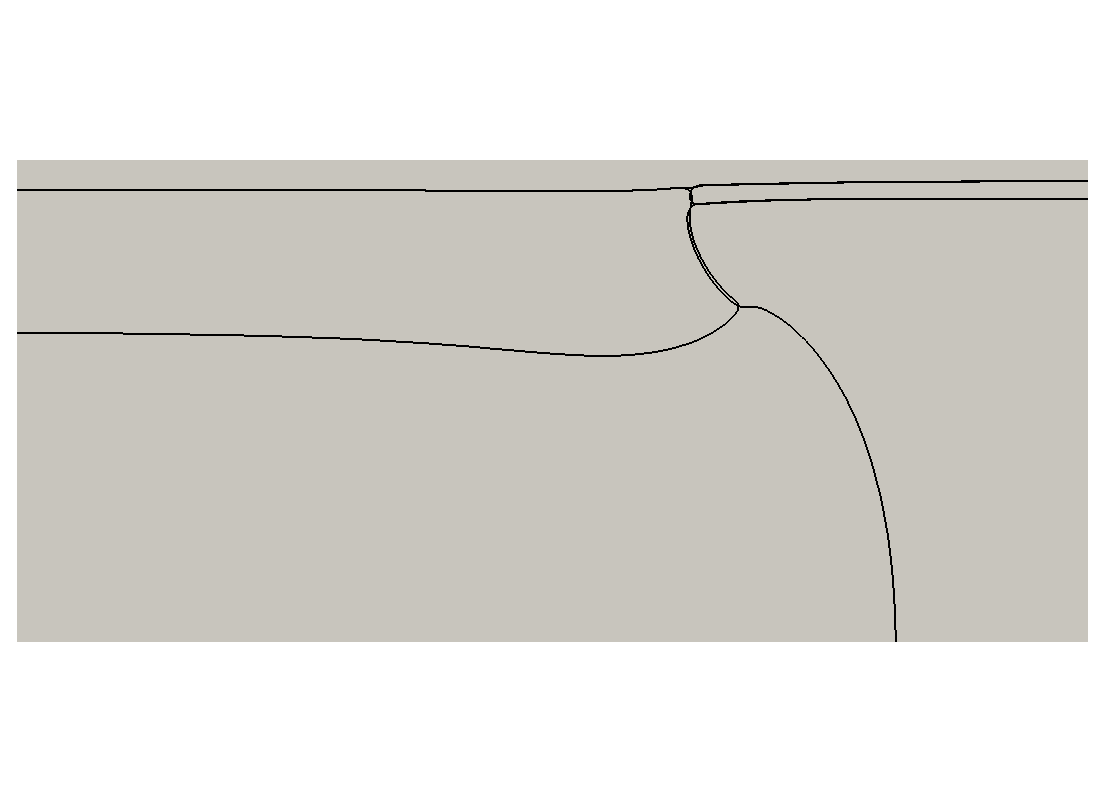
\includegraphics[width=3.25cm]{python_codes/fieldstone_118/results/case1/c}
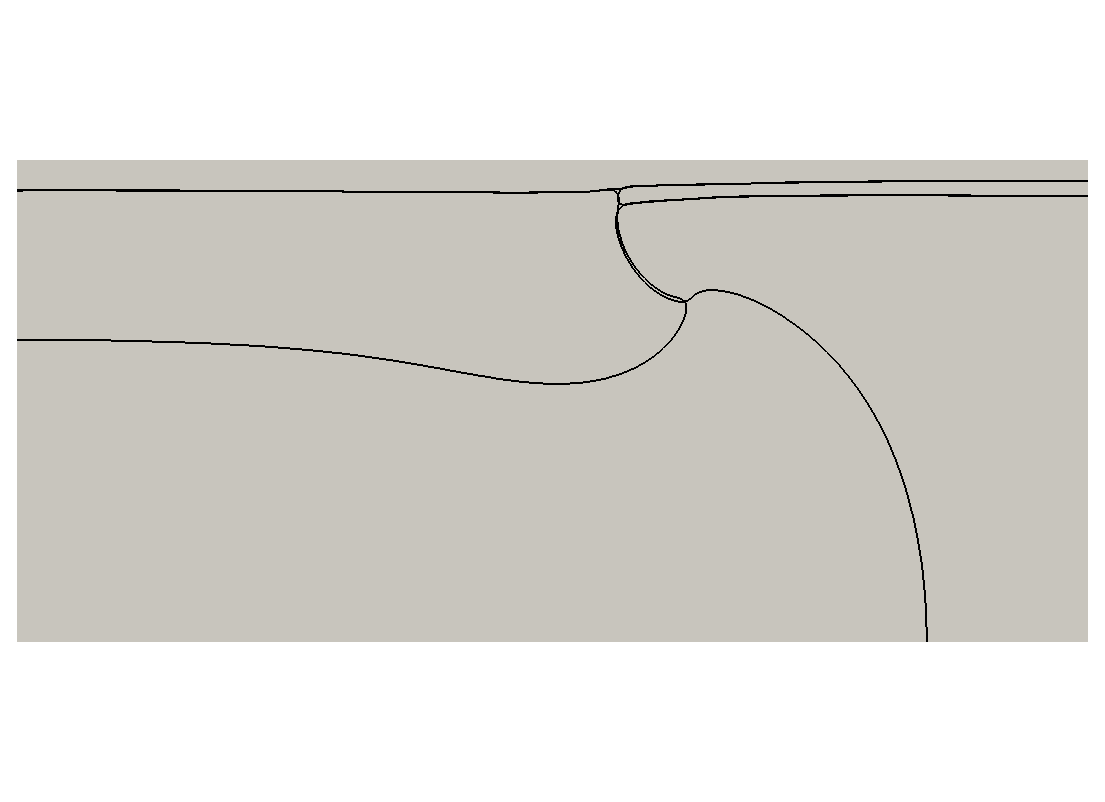
\includegraphics[width=3.25cm]{python_codes/fieldstone_118/results/case1/d}
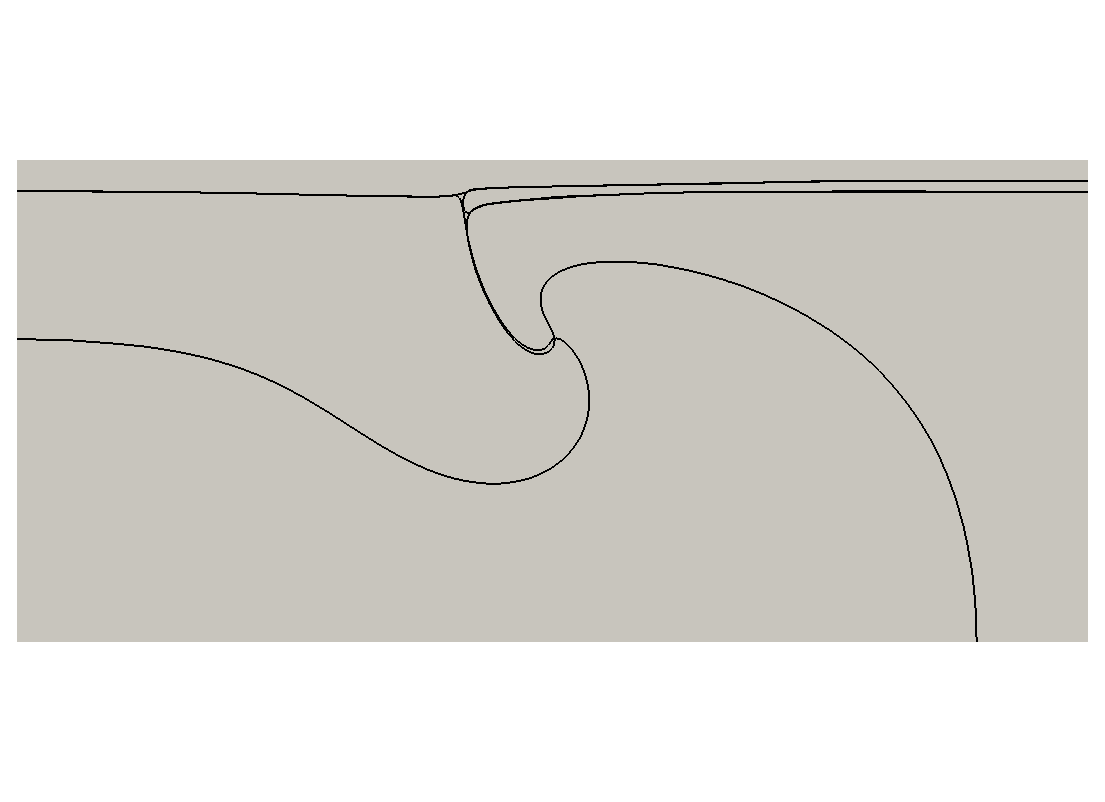
\includegraphics[width=3.25cm]{python_codes/fieldstone_118/results/case1/e}\\
{\captionfont System at times 0, 10, 20, 30 and 50~Myr.}
\end{center}


\begin{center}
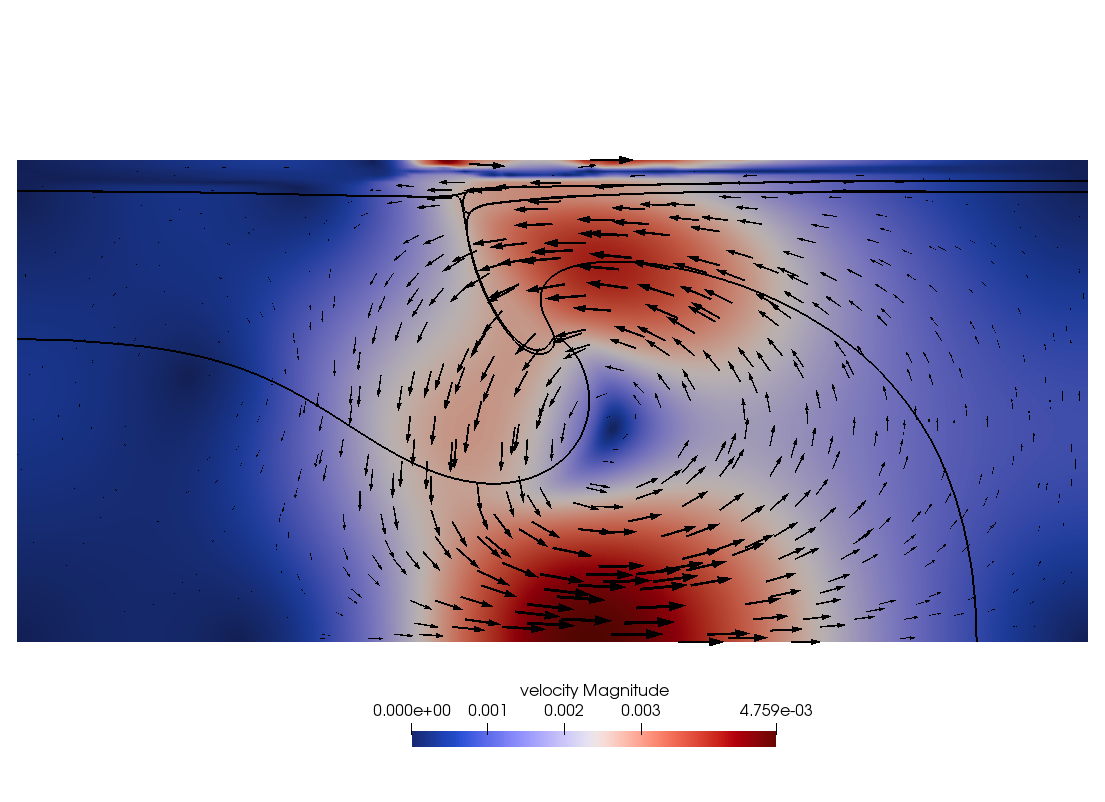
\includegraphics[width=4cm]{python_codes/fieldstone_118/results/case1/vel}
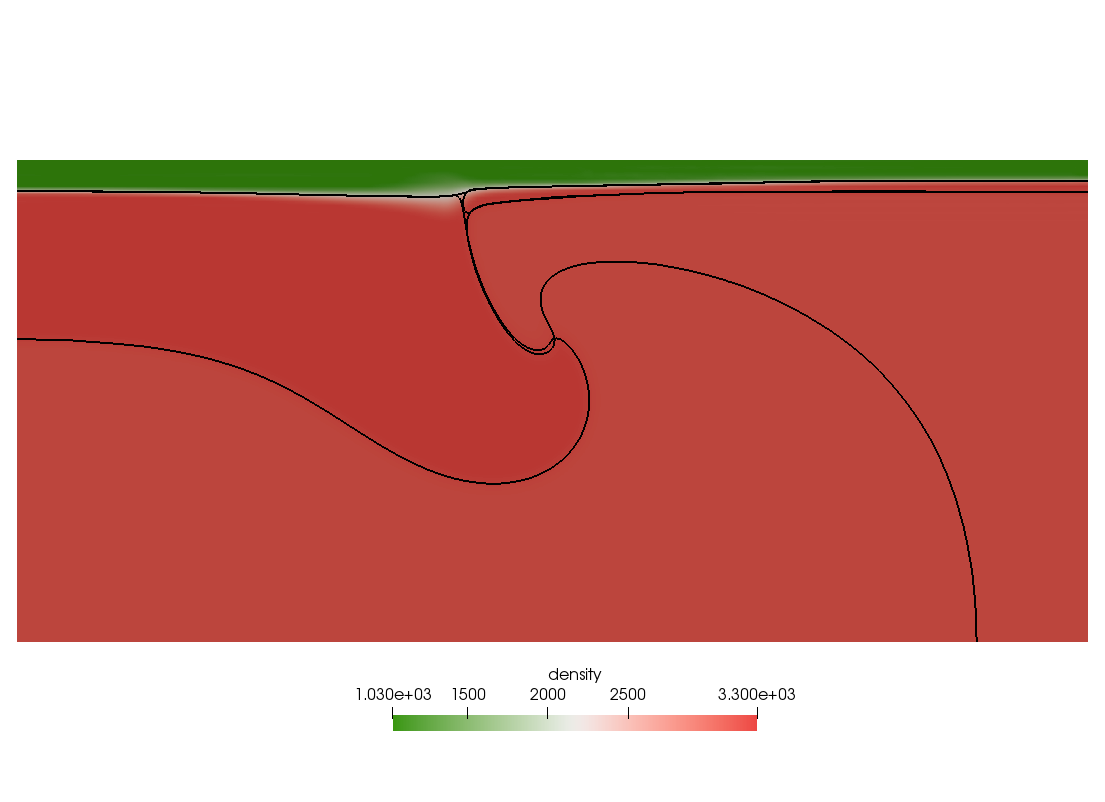
\includegraphics[width=4cm]{python_codes/fieldstone_118/results/case1/rho}
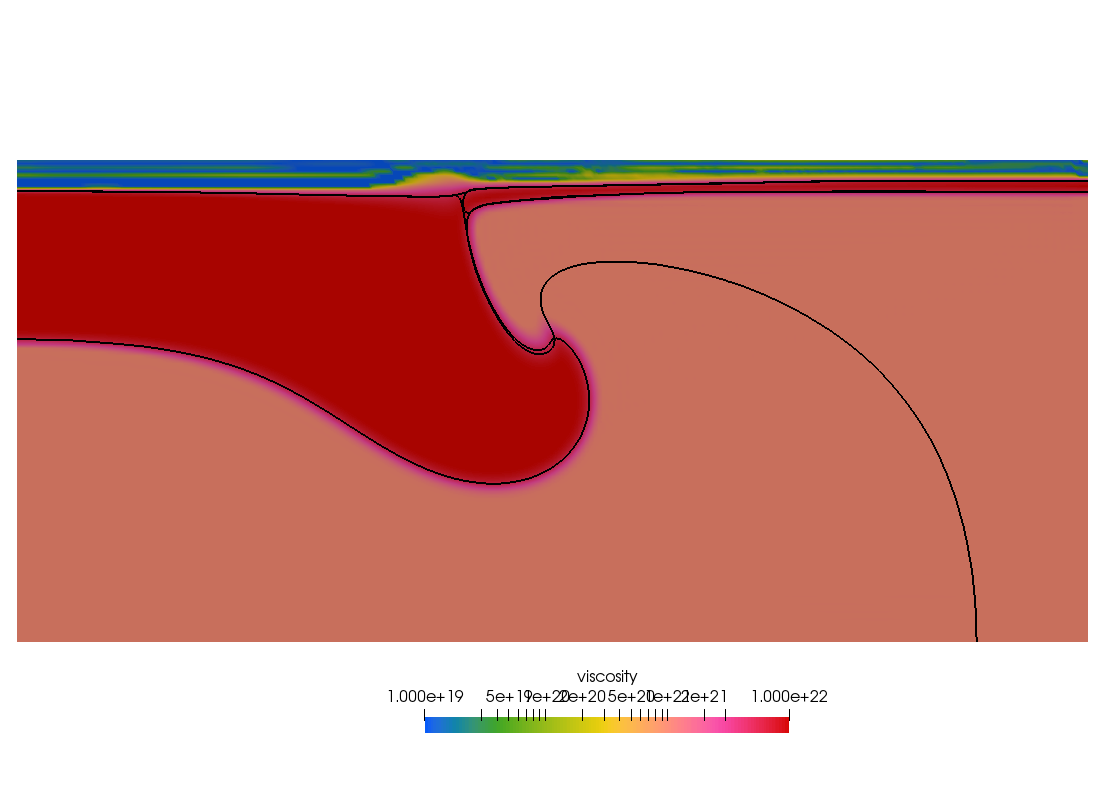
\includegraphics[width=4cm]{python_codes/fieldstone_118/results/case1/eta}
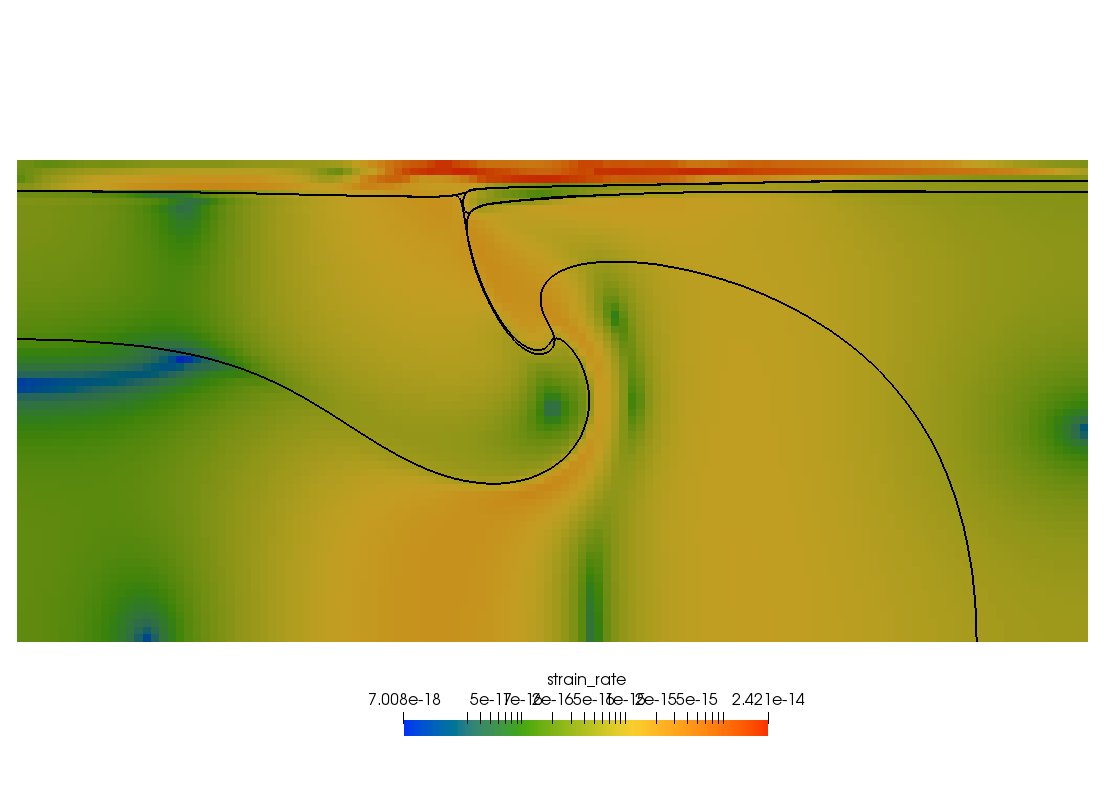
\includegraphics[width=4cm]{python_codes/fieldstone_118/results/case1/sr}\\
{\captionfont Various fields at $t=50$ Myr.}
\end{center}

%%%%%%%%%%%%%%%%%%%%%%%%%%%%%%%%%%%%%%%%%%%%%%%%%%%%%%%%%%%%%%%%%%%%%%%
\subsection*{Results - Case 1* }

This case is not in the original publication. It consists of Case 1 run with a 
50\% longer domain, all other things equal (with $L_0=2L_x/3$). We find that the domain size does not
play a large role in the model evolution at all: 

\begin{center}
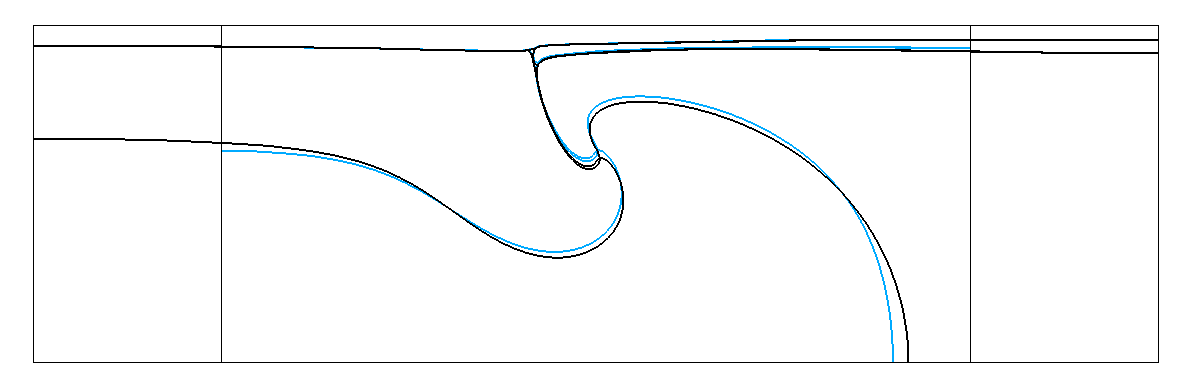
\includegraphics[width=9cm]{python_codes/fieldstone_118/results/case1b/isos}\\
{\captionfont Compositional fields isolines at $t=50$ Myr. Black lines correspond
to 600x180 domain while blue lines correspond to 400x180km domain.}
\end{center}

%%%%%%%%%%%%%%%%%%%%%%%%%%%%%%%%%%%%%%%%%%%%%%%%%%%%%%%%%%%%%%%%%%%%%%%
\subsection*{Results - Case 2}

\begin{center}
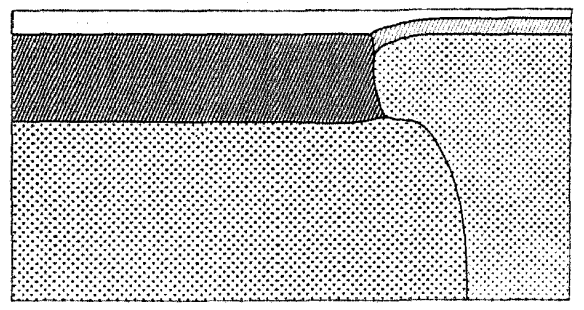
\includegraphics[width=3.25cm]{python_codes/fieldstone_118/images/case2/a}
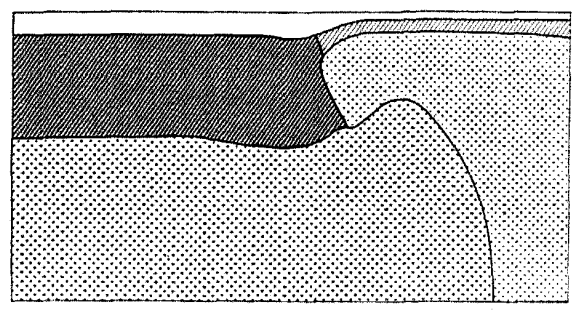
\includegraphics[width=3.25cm]{python_codes/fieldstone_118/images/case2/b}
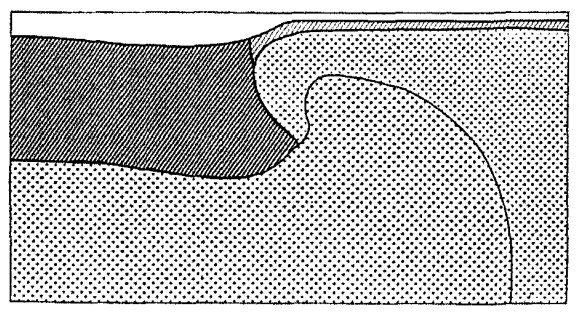
\includegraphics[width=3.25cm]{python_codes/fieldstone_118/images/case2/c}\\
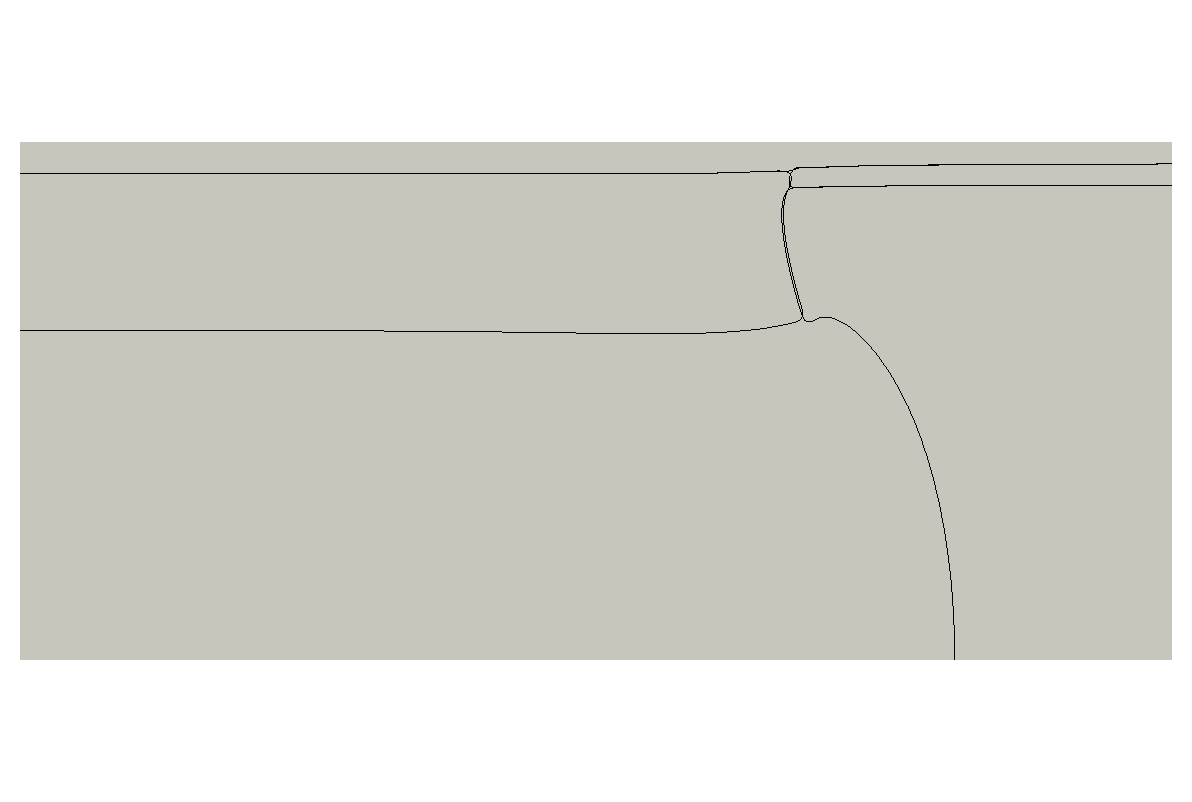
\includegraphics[width=3.25cm]{python_codes/fieldstone_118/results/case2/a}
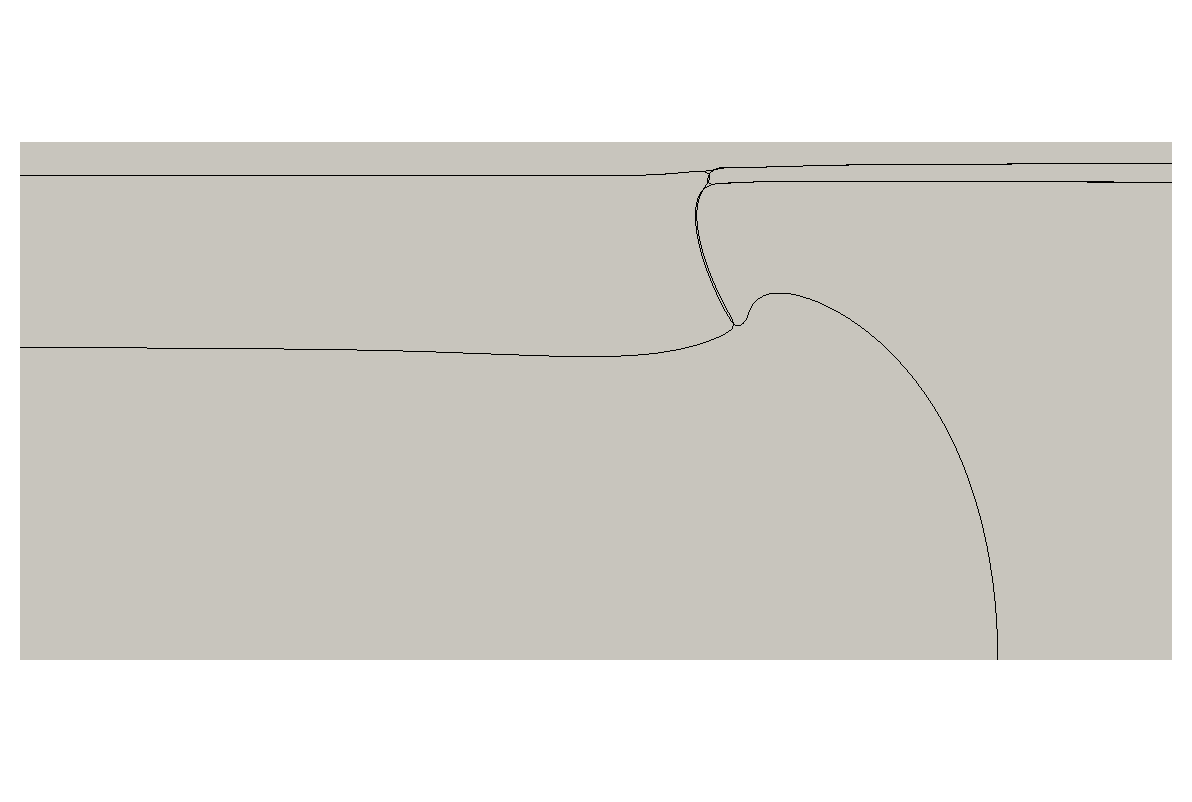
\includegraphics[width=3.25cm]{python_codes/fieldstone_118/results/case2/b}
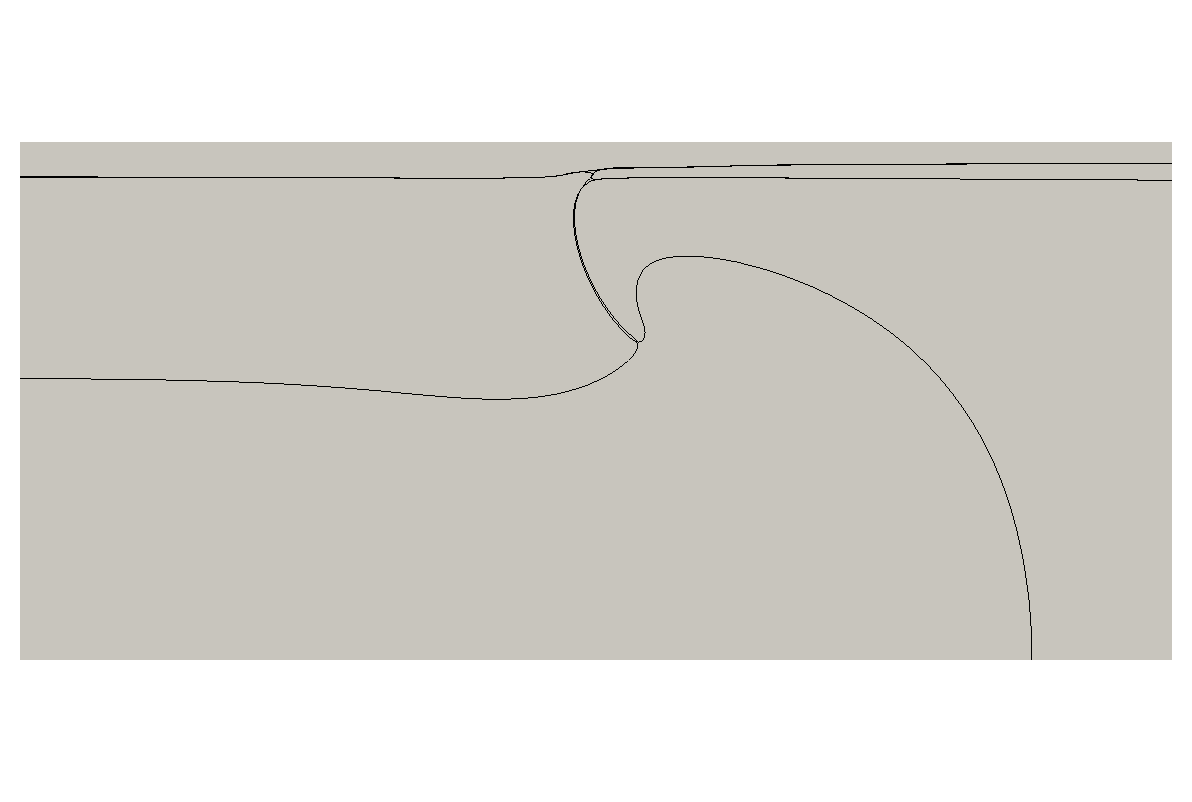
\includegraphics[width=3.25cm]{python_codes/fieldstone_118/results/case2/c}\\
{\captionfont System at times 9.6, 16.6 and 25.1~\si{\mega\year}.}
\end{center}

\begin{center}
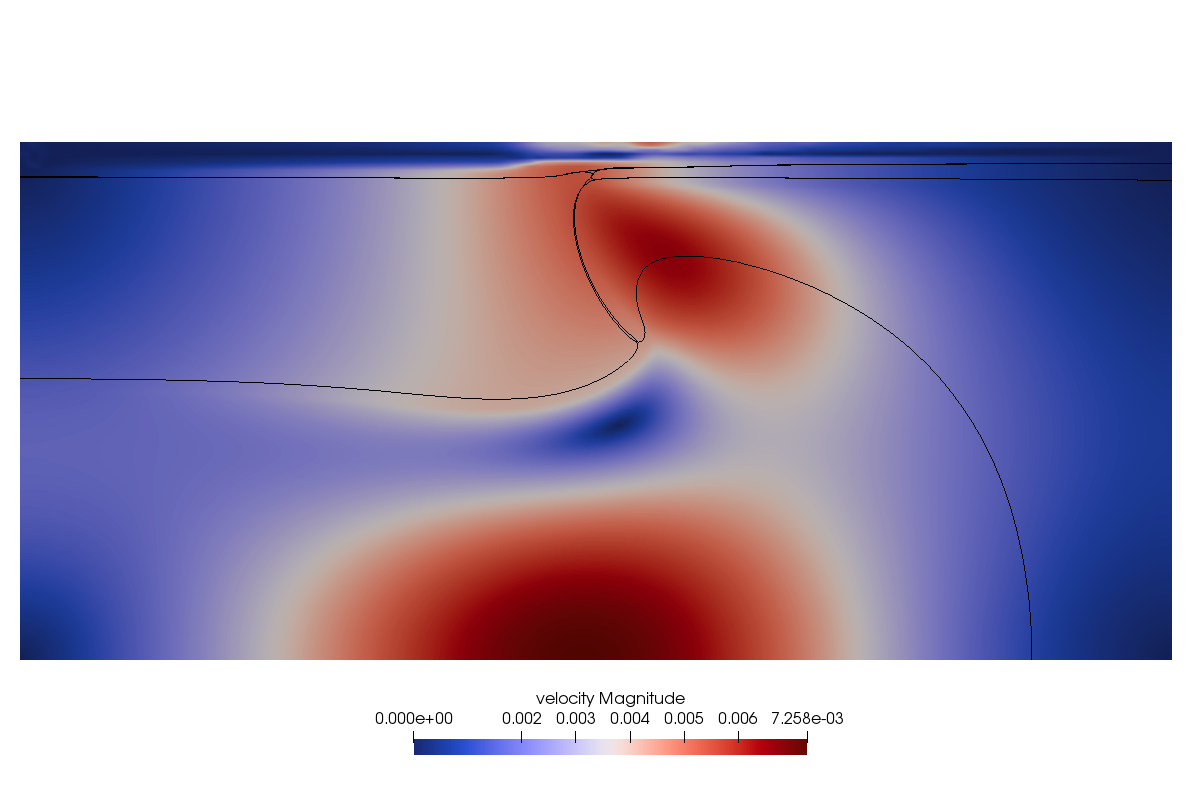
\includegraphics[width=4cm]{python_codes/fieldstone_118/results/case2/vel}
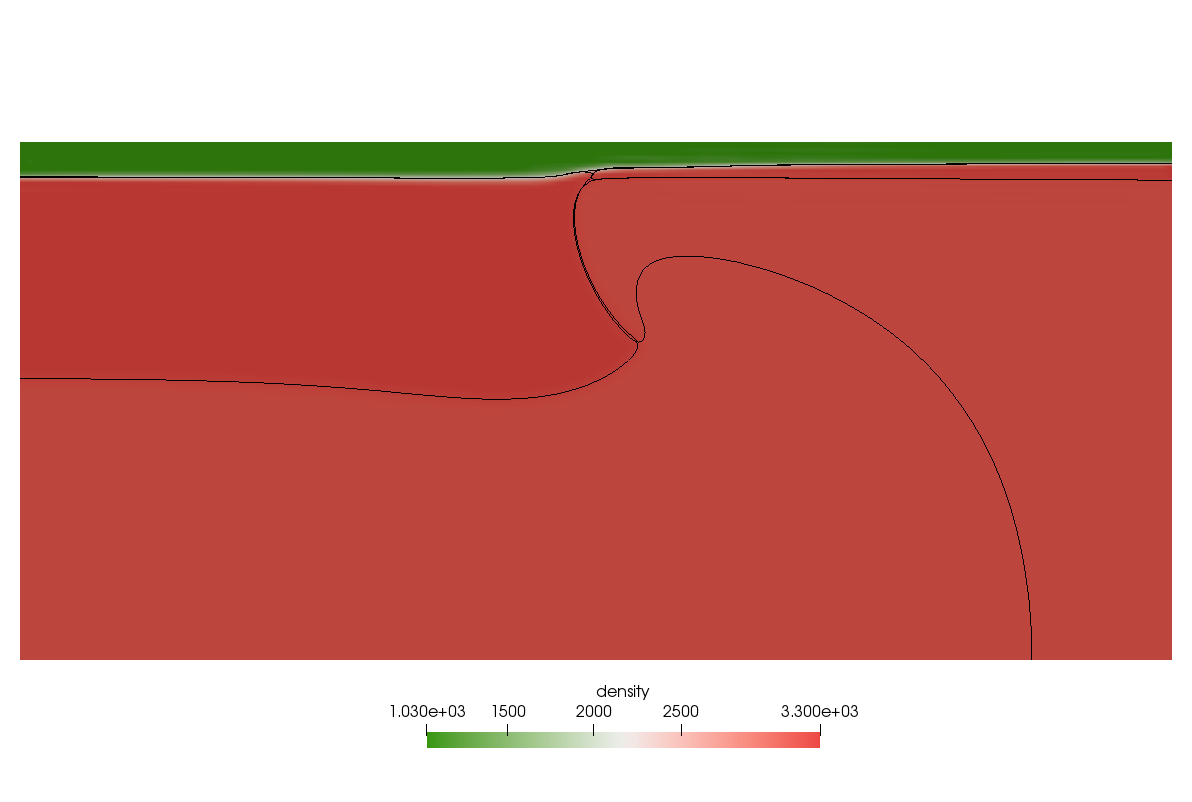
\includegraphics[width=4cm]{python_codes/fieldstone_118/results/case2/rho}
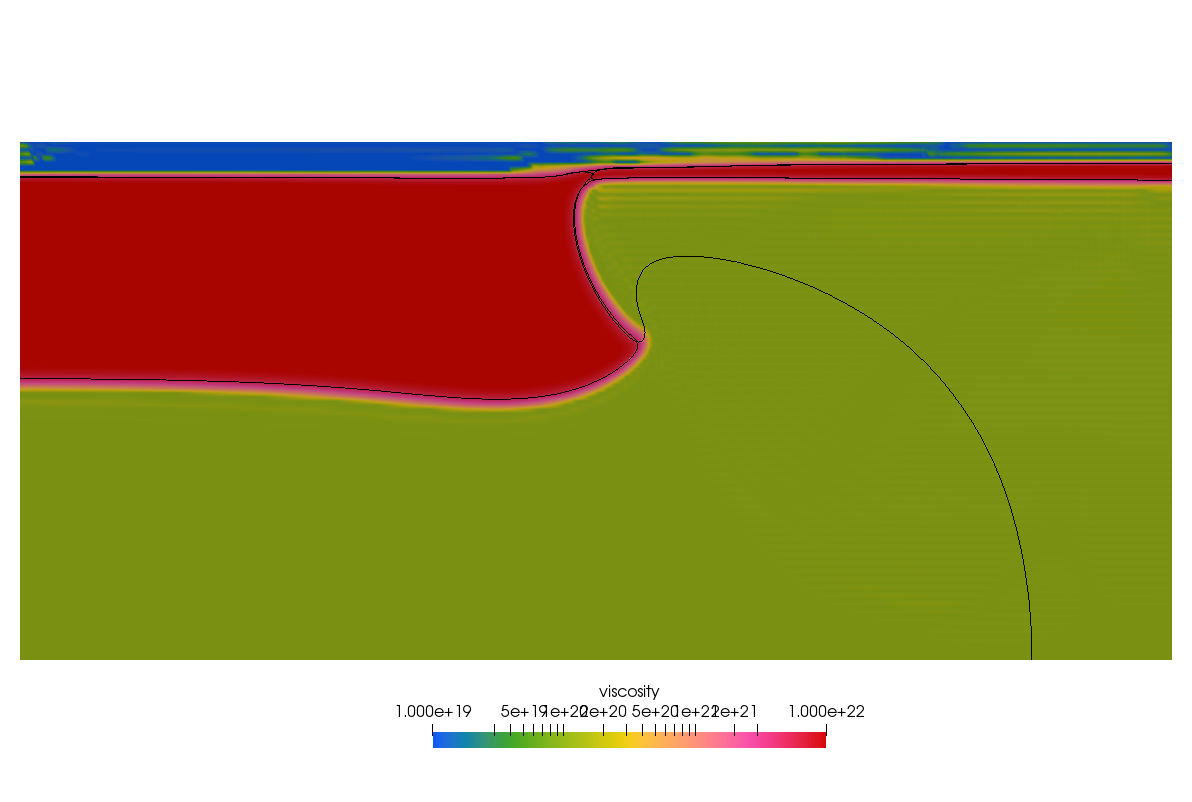
\includegraphics[width=4cm]{python_codes/fieldstone_118/results/case2/eta}
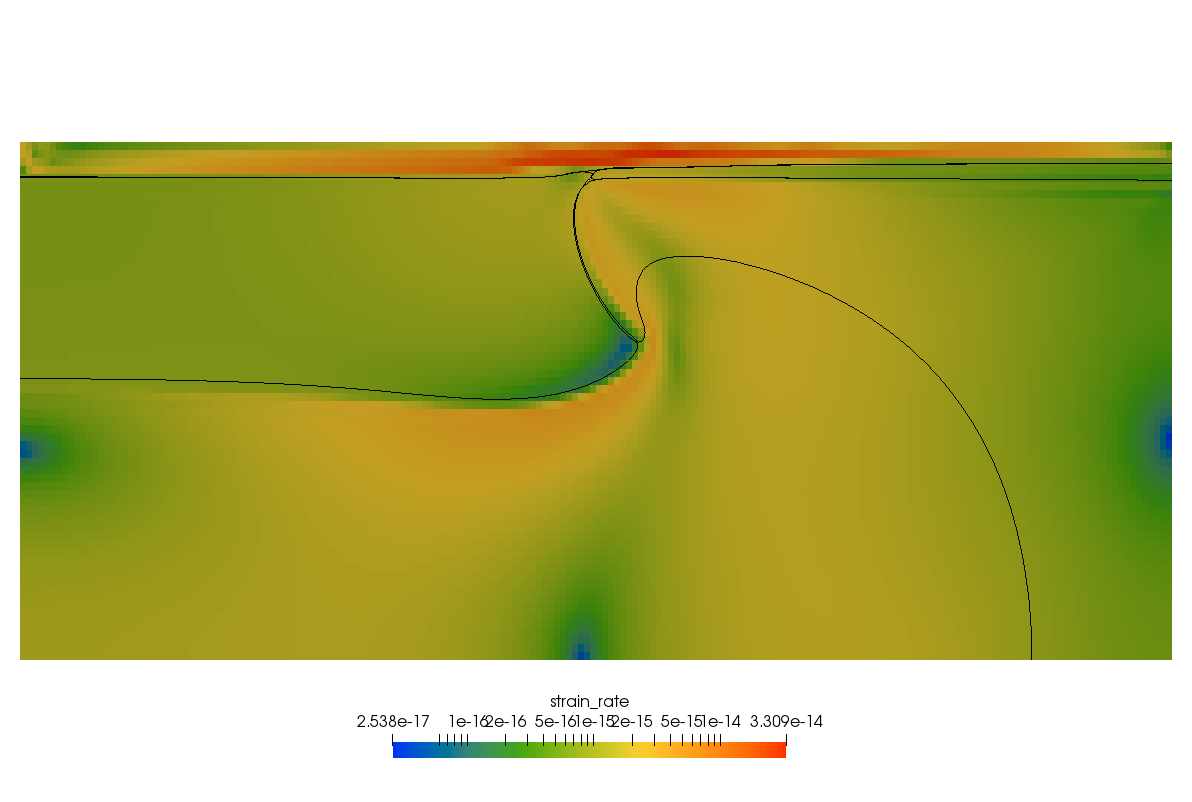
\includegraphics[width=4cm]{python_codes/fieldstone_118/results/case2/sr}\\
{\captionfont Various fields at $t=25.1~\si{\mega\year}$.}
\end{center}



TODO: run stone 67 with pic!

